\documentclass[../main/main.tex]{subfiles}
\graphicspath{{./figures/}}

\makeatletter
\renewcommand{\@chapapp}{Travaux pratiques -- TP}
\makeatother

% \toggletrue{student}
% \toggletrue{corrige}
% \renewcommand{\mycol}{black}
% \renewcommand{\mycol}{gray}

\hfuzz=5.002pt

\begin{document}
\setcounter{chapter}{24}

\settype{enon}
\settype{solu_prof}
\settype{solu_stud}

\chapter{\cswitch{%
	  Correction du TP
  }{%
	  Exploitation des $E-\pH$~: méthode de \textsc{Winkler}%
  }%
 }

\enonce{%
	% \begin{tcn}*(exem)<ctc>{\iconhow~Capacités exigibles}
	% 	\begin{itemize}
	% 		\item Mettre en œuvre un protocole expérimental correspondant à un titrage
	% 		      indirect.
	% 		\item Justifier la nécessité de faire un titrage indirect.
	% 		\item Choisir et utiliser un indicateur coloré de fin de
	% 		      titrage~; distinguer l'équivalence et le virage d'un indicateur
	% 		      coloré de fin de titrage.
	% 		\item Mettre en œuvre une démarche expérimentale s'appuyant sur
	% 		      l'utilisation d'un diagramme potentiel-$\pH$.
	% 	\end{itemize}
	% \end{tcn}
	% \vspace{-10pt}
	%
	\section{Objectifs}

	\begin{itemize}
		\item Savoir exploiter un diagramme $E-\pH$ fourni, et la superposition de
		      plusieurs diagrammes.
		\item Déterminer la concentration en dioxygène dissous $[\ce{{O_2}_{\gaz}}]$
		      dans l'eau du robinet par titrage colorimétrique redox.
	\end{itemize}

	\section{S'approprier}
	\subsection{Introduction}
	La teneur en dioxygène est significative de la qualité biologique d'une eau~:
	\begin{itemize}
		\item Les \textbf{eaux pollués} renferment \textbf{peu ou pas} de dioxygène
		      dissous, parce que les micro-organismes qui font fermenter les déchets
		      organique consomment cet oxygène massivement.
		\item Les eaux \textbf{non polluées} renferment des \textbf{quantités
			      importantes} de dioxygène parce que le gain du dioxygène par la
		      dissolution de ce gaz en surface ainsi que par la photosynthèse des
		      plantes aquatiques est plus important que sa perte par la putréfaction des
		      rares déchets.
	\end{itemize}
	\subsection{Titrage du taux de dioxygène dissous}
	Comme le dioxygène est un oxydant, on peut songer à réaliser un titrage par
	oxydo-réduction. Or, il n'existe pas de réducteur qui à la fois change de
	couleur en passant à l'état oxydé \textbf{et} qui réagisse suffisamment vite
	avec l'oxygène. Il faudra donc opérer par voie détournée. On utilise ici la
	méthode de \textsc{Winkler}.
	\bigbreak
	On oxyde du manganèse II par le dioxygène dissous  dans l'eau en milieu
	basique. Le manganèse précipite alors en $\ce{{Mn(OH)_3}_{\sol}}$. Cette
	réaction est lente. En milieu suffisamment acide, ce précipité peut oxyder des
	ions iodure en excès. Finalement, on dose l'iode ainsi formée par une solution
	de thiosulfate, en présence d'empois d'amidon (la coloration bleue de l'amidon
	en présence d'iode disparaît au virage).
}

\setcounter{section}{2}
\section{Analyser}
\subsection{Diagrammes $E-\pH$}
\enonce{%
On donne ci-après les diagrammes à compléter $E-\pH$ du manganèse et de l'iode.
Les espèces présentes sont $\ce{Mn^{2+}_{\aqu}}$, $\ce{Mn^{3+}_{\aqu}}$,
$\ce{{Mn(OH)_2}_{\sol}}$ et $\ce{{Mn(OH)_3}_{\sol}}$ pour le premier, et
$\ce{{I_2}_{\aqu}}$, $\ce{I^-_{\aqu}}$ et $\ce{{IO_3}^{-}_{\aqu}}$ pour le
second. La convention de tracé est $c_t = \SI{e-2}{mol.L^{-1}}$ en chaque
élément.
}%

\setlist[blocQR,1]{leftmargin=10pt, label=\clenumi}
\QR{%
	Attribuer chaque zone à l'espèce correspondante.
}{%
	On analyse les \no et on étudie l'acido-basicité des espèces. On trouve le
	résultat Figure~\ref{fig:eph_mg}.
}%
\QR{%
Superposer le diagramme du couple $\ce{{O_2}_{\aqu}/H_2O_{\liq}}$, avec la
même convention de tracé.
}{%
Idem. Attention, cette fois $a(\ce{O_2}) = [\ce{O_2}]$, donc à la frontière on
a $[\ce{O_2}] = \SI{e-2}{mol.L^{-1}}$ et $\log
	\frac{[\ce{O_2}]\ind{front}}{c^\circ} = -2$.
}%

\begin{center}
	\cswitch{
		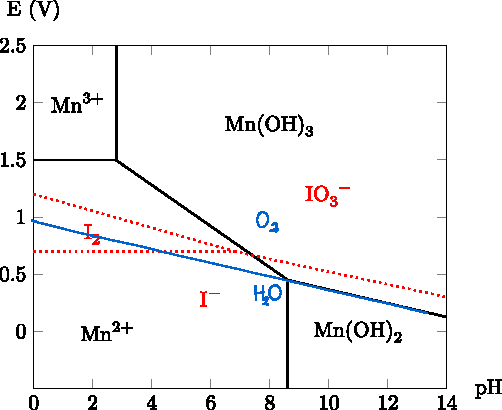
\includegraphics[width=.5\linewidth]{eph_mg-eau}
	}{
		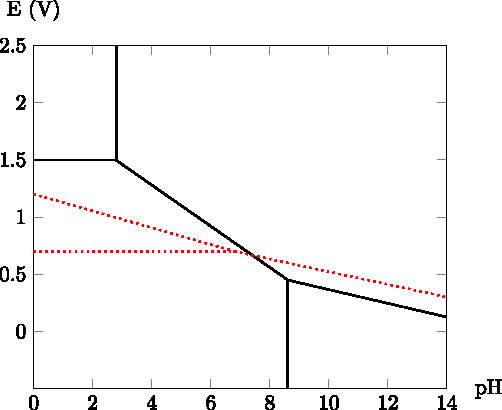
\includegraphics[width=.5\linewidth]{eph_mg-plain}
	}
	\captionof{figure}{Diagrammes $E-\pH$ du manganèse en traits plein, de l'iode
		en pointillés.}
	\label{fig:eph_mg}
\end{center}

\subsection{Oxydation du manganèse par le dioxygène}
\enonce{%
	Dans un erlenmeyer rempli d'eau du robinet, on ajoute \SI{1}{g} de soude, puis
	environ \SI{2}{g} de sulfure de manganèse $\ce{{MnSO_4}_{\sol}}$, qui est très
	soluble dans l'eau.
}%
\QR{%
	Écrire la réaction de dissolution du solide dans l'eau, puis l'équation-bilan
	(1) acido-basique de l'action de la soude sur cette solution.
}{%
	\leavevmode\vspace*{-25pt}\relax
	\begin{align*}
		\ce{{MnSO_4}_{\sol}                  & = Mn^{2+}_{\aqu} + {SO_4}^{2-}_{\aqu}}
		\tag*{dissolution}
		\\
		\ce{Mn^{2+}_{\aqu} + 2 {HO}^-_{\aqu} & = {Mn(OH)_2}_{\sol}}
		\tag{1}
	\end{align*}
}%
\QR{%
	Écrire l'équation bilan (2) redox de l'action du dioxygène dissous sur le
	précipité obtenu. Justifier la nécessité d'un milieu réactionnel basique ainsi
	que le caractère total de cette réaction à l'aide du diagramme potentiel-\pH.
}{%
	\leavevmode\vspace*{-25pt}\relax
	\begin{align*}
		\ce{2H_2O_{\liq}                    & = {O_2}_{\aqu} + 4H^+_{\aqu} + 4e^-}
		\tag{R1}
		\\
		\ce{{Mn(OH)_2}_{\sol} + H_2O_{\liq} & = {Mn(OH)_3}_{\sol} + H^+_{\aqu} + e^-}
		\tag{R2}
		\\\Ra
		\ce{
		4 {Mn(OH)_2}_{\sol} + {O_2}_{\aqu}} +
		\underbracket[1pt]{\cancel{4}}_{2}\ce{H2O_{\liq} + \bcancel{\ce{4H^+_{\aqu}}}
		                                    & =
		\cancel{\ce{2H_2O_{\liq}}} + 4{Mn(OH)_3}_{\sol} + \bcancel{\ce{4H^+_{\aqu}}}
		}
		\tag*{$\rm 4(R2)-(R1)$}
		\\\Lra
		\ce{
		4 {Mn(OH)_2}_{\sol} + {O_2}_{\aqu} +
		2H2O_{\liq}
		                                    & =
		4{Mn(OH)_3}_{\sol}
		}
		\tag{2}
		\label{eq:2}
	\end{align*}
	On se met en milieu basique pour éviter l'obtention de $\ce{Mn^{2+}}$ ou
	$\ce{Mn^{3+}}$. Sur le diagramme, on voit que les domaines sont séparés d'au
	moins \SI{0.20}{V}, donc la réaction est bien totale.
}%
\QR{%
	Sachant que la solubilité du dioxygène est de l'ordre de \SI{40}{mg.L^{-1}}
	dans l'eau à \SI{25}{\degreeCelsius}, justifier que le dioxygène est bien le
	réactif limitant de la réaction (2).
}{%
	solu
}%

\subsection{Acidification du milieu}
\enonce{%
	Quand l'oxydation par le dioxygène est terminée, on ajoute \SI{1}{mL} d'acide
	sulfurique concentré.
}%
\QR{%
	Écrire les équations bilan (3) et (3') acido-basiques de l'action de l'acide
	sur le manganèse III formé précédemment et l'excès de manganèse II restant.
}{%
	\leavevmode\vspace*{-25pt}\relax
	\begin{gather}
		\ce{{Mn(OH)_3}_{\sol} + 3H^+_{\aqu} = Mn^{3+}_{\aqu} + 3H_2O_{\liq}}
		\tag{3}
		\label{eq:3}
		\\
		\ce{{Mn(OH)_2}_{\sol} + 2H^+_{\aqu} = Mn^{2+}_{\aqu} + 2H_2O_{\liq}}
		\tag{3'}
	\end{gather}
}%
\QR{%
	Pourquoi faut-il passer en milieu acide avant l'ajout des ions
	$\ce{I^-}_{\aqu}$~?
}{%
	Sinon on ne formera pas le diiode que l'on veut titrer~!
}%
\QR{%
	À l'aide des diagrammes $E-\pH$, montrer qu'en milieu très acide le dioxygène
	de l'air ne peut plus oxyder le manganèse II en manganèse III. Est-il
	nécessaire de boucher l'erlenmeyer dans la suite~?
}{%
	En milieu basique, les ions $\ce{Mn^{2+}_{\aqu}}$ ont un domaine commun avec
	$\ce{{O_2}_{\aqu}}$~: ils ne réagissent pas ensemble. Ainsi, étant donné qu'on
	a précédemment consommé tout le dioxygène pour former du manganèse III, il n'y
	a pas de risque à ce que du dioxygène soit re-dissout en solution~: ce n'est
	pas lui que l'on va titrer et il ne réagit pas avec les espèces d'intérêt. On
	peut laisser le bouchon ouvert.
}%

\subsection{Réduction du manganèse par l'iode}
\enonce{%
	On ajoute ensuite \SI{3}{g} d'iodure de potassium $\ce{KI}$ solide.
}%
\QR{%
	Écrire l'équation-bilan (4) redox correspondant à l'action des ions \ce{I^-}
	sur la solution. Justifier le caractère total de cette réaction par lecture du
	diagramme $E-\pH$.
}{%
	\leavevmode\vspace*{-25pt}\relax
	\begin{align*}
		\ce{Mn^{2+}_{\aqu}                   & = Mn^{3+} + e^-}
		\tag{R3}
		\\
		\ce{2I^{-}_{\aqu}                    & = {I_2}_{\aqu} + 2e^-}
		\tag{R4}
		\\\Ra
		\beforetext{(R4)$-$2(R3) $\Ra$}
		\ce{2Mn^{3+}_{\aqu} + 2 I^{-}_{\aqu} & = 2Mn^{2+}_{\aqu} + {I_2}_{\aqu}}
		\tag{4}
		\label{eq:4}
	\end{align*}
	L'écart de potentiel est d'environ \SI{1}{V} en milieu basique, donc la
	réaction est bien totale.
}%
\QR{%
	Justifier que \ce{I^-} soit le réactif en excès.
}{%
	Comme précédemment, le réactif limitant était \ce{O2} qui donnaît
	\ce{4Mn(OH)3}, lui-même donnant totalement des \ce{Mn^3+}. Avec \SI{3}{g}
	d'iodure de potassium, on a…
	% TODO: Finir le calcul
}%

\subsection{Titrage du diiode par le thiosulfate}
\enonce{%
	On prélève un volume $V_0 = \SI{100}{mL}$ de la solution de l'erlenmeyer pour
	le doser par une solution de thiosulfate de sodium $(2
		\ce{Na^+}~;~\ce{{S_2O_3}^{2-}})$ de concentration en ions thiosulfate égale à
	$c_0 = \SI{1.3e-2}{mol.L^{-1}}$. On note $V\ind{eqv}$ le volume équivalent.
}%
\QR{%
	Écrire les deux demi-équations redox mises en jeu et en déduire la réaction
	(5) support du dosage. On admet qu'elle est quantitative.
}{%
	\leavevmode\vspace*{-20pt}\relax
	\begin{align*}
		\ce{2 {S_2O_3}^2-_{\aqu}              & = {S_4O_6}^2-_{\aqu} + 2e^-}
		\tag{R5}
		\\
		\ce{2 {I}^-_{\aqu}                    & = {I_2}_{\aqu} + 2e^-}
		\tag{R6}
		\\
		\beforetext{(R5)$-$(R6) $\Ra$}
		\ce{
		{I_2}_{\aqu} + 2 {S_2O_3}^{2-}_{\aqu} & = 2 {I}^-_{\aqu} +
		{S_4O_6}^{2-}_{\aqu}
		}
		\tag{5}
	\end{align*}
}%
\QR{%
	Déterminer la relation en $n(\ce{I_2})$, $c_0$ et $V\ind{eqv}$.
}{%
	\leavevmode\vspace*{-15pt}\relax
	\label{q:ni2}%
	\begin{center}
		\def\rhgt{0.35}
		\centering
		\begin{tabularx}{\linewidth}{|l|c||YdYdYdY|}
			\hline
			\multicolumn{2}{|c||}{
				$\xmathstrut{\rhgt}$
			\textbf{Équation}}           &
			$\ce{{I_2}_{\aqu}}$          & $+$                  &
			$2\ce{{S_2O_3}^{2-}_{\aqu}}$ & $\ra$                &
			$2\ce{{I}^-_{\aqu}}$         & $+$                  &
			$\ce{{S_4O_6}^{2-}}$                                  \\
			\hline
			$\xmathstrut{\rhgt}$
			Initial                      & $\xi = 0$            &
			$n(\ce{I_2})$                & \vline               &
			$c_0V$                       & \vline               &
			$0$                          & \vline               &
			$0$                                                   \\
			\hline
			$\xmathstrut{\rhgt}$
			Interm.                      & $\xi$                &
			$n(\ce{I_2}) - \xi$          & \vline               &
			$c_0V - 2\xi$                & \vline               &
			$2\xi$                       & \vline               &
			$\xi$                                                 \\
			\hline
			$\xmathstrut{\rhgt}$
			Équiv.                       & $\xi_f = \xi_{\max}$ &
			$0$                          & \vline               &
			$0$                          & \vline               &
			$2c_0V\ind{eqv}$             & \vline               &
			$c_0V\ind{eqv}$                                       \\
			\hline
		\end{tabularx}
	\end{center}
	\vspace{-15pt}
	\begin{gather*}
		\beforetext{À l'équivalence,}
		\xi_f = \xi\ind{max}
		\Lra
		\boxed{n(\ce{I_2}) = \frac{c_0V_{\eqi}}{2}}
	\end{gather*}
}%
\QR{%
	En utilisant les équations (4), (3) et (2), déterminer les relations entre
	$n(\ce{Mn^{3+}})$ et $n(\ce{I_2})$ d'une part, puis entre
	$n(\ce{{Mn(OH)_3}_{\sol}})$ et $n(\ce{I_2})$ d'autre part, et finalement entre
	$n(\ce{{Mn(OH)_3}_{\sol}})$ et $n(\ce{{O_2}_{\aqu}})$.
}{%
	\begin{itemize}
		\item
		      \leftcenters{%
			      \eqref{eq:4} totale, donc
		      }{%
			      $\DS\frac{n(\ce{Mn^{3+}})}{2} = n(\ce{I_2})$
		      }%
		\item
		      \leftcenters{%
			      \eqref{eq:3} totale, donc
		      }{%
			      $n(\ce{{Mn(OH)_3}_{\sol}}) = n(\ce{Mn^{3+}}) = 2n(\ce{I_2})$
		      }%
		\item
		      \leftcenters{%
			      \eqref{eq:2} totale, donc
		      }{%
			      $n(\ce{{Mn(OH)_3}_{\sol}}) = 4n(\ce{O_2})$
		      }%
	\end{itemize}
}%
\QR{%
	En déduire la relation entre $n(\ce{O_2})$ et $n(\ce{I_2})$, puis montrer qu'à
	l'équivalence on a donc
	\[
		[\ce{{O_2}_{\aqu}}]  = \frac{c_0V\ind{eqv}}{4V_0}
	\]
}{%
	\leavevmode\vspace*{-25pt}\relax
	\begin{gather*}
		4 n(\ce{O_2}) = 2 n(\ce{I_2}) \Lra n(\ce{O_2}) = \frac{n(\ce{I_2})}{2}
		\\\beforetext{\ref{q:ni2} $\Ra n(\ce{I_2}) = \frac{c_0V\ind{eqv}}{2}$}
		\Lra
		\boxed{[\ce{{O_2}_{\aqu}}] = \frac{c_0V\ind{eqv}}{4V_0}}
	\end{gather*}
}%

\subsection{Bilan~: au travers du diagramme}
\QR{%
	Reprendre le diagramme $E-\pH$ avec le manganèse, l'iode et l'eau, et faire
	figurer sur ce diagramme chacune des étapes précédentes. Représenter les
	étapes par des croix et les réactions entre composés par des flèches.
}{%
	\sswitch{
		\hfill
		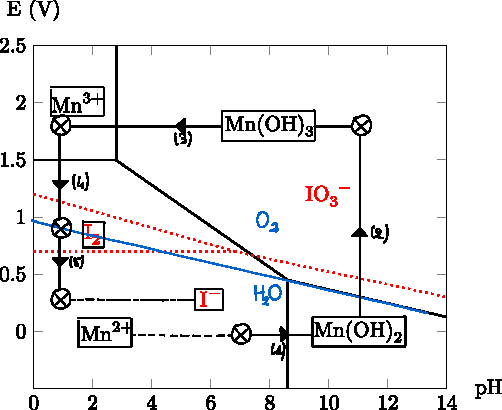
\includegraphics[width=.6\linewidth, valign=t]{eph_mg-chemin}
		\hspace*{\fill}
	}{
		\leavevmode\vspace*{-15pt}\relax
		\begin{center}
			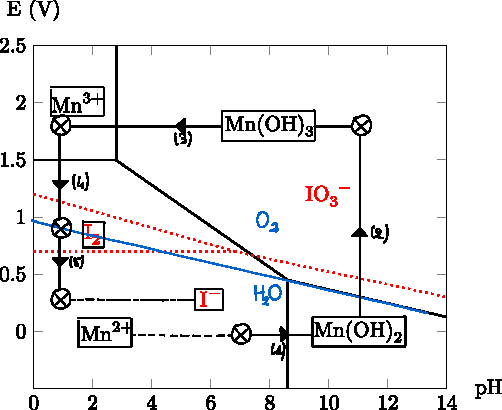
\includegraphics[width=.6\linewidth]{eph_mg-chemin}
		\end{center}
	}
}%

\section{Réaliser}
\enonce{%
	\begin{tcn}*[breakable](prop)"bomb"{Attention}
		\begin{itemize}
			\item Vous manipulez de la soude et de l'acide sulfurique très concentrés~:
			      il est impératif de porter des lunettes, des gants \textbf{et
				      d'avoir les jambes couvertes}.
			\item Tout contact avec les yeux ou la peau est sérieusement dangereux. En
			      cas de contact, laver immédiatement et très abondammant à l'eau.
			\item Attention à ne pas en mettre sur votre paillasse. Si c'est le cas,
			      nettoyer immédiatement. Prenez soin de manipuler dans un
			      \textbf{espace adapté}.
		\end{itemize}
	\end{tcn}
}%

\subsection{Oxydation du manganèse par le dioxygène}
\enonce{%
	\begin{tcb}*(expe)<itc>"chem"{Oxydation du manganèse}
		\begin{enumerate}
			\item Placer un erlenmeyer de volume \SI{250}{mL} dans un cristallisoir, en
			      prévision de débordements de liquide corrosif. Y placer un barreau
			      aimanté et \SI{1}{g} de soude, en la manipulant avec des gants.
			      Ajouter ensuite environ \SI{2}{g} de sulfate de manganèse solide.

			\item Remplir totalement d'eau du robinet. \textbf{Boucher aussitôt
				      l'erlenmeyer} sans laisser aucune bulle d'air entre le bouchon et le
			      niveau d'eau~: Le dioxygène de l'air pourrait alors se dissoudre dans
			      l'eau et fausserait le résultat.

			\item Agiter périodiquement (une agitation continue n'est pas nécessaire)
			      et énergiquement pendant une vingtaine de minutes.
		\end{enumerate}
	\end{tcb}
}%

\resetQ
\setlist[blocQR,1]{leftmargin=10pt, label=\sqenumi}
\QR{%
	Noter l'aspect du contenu de l'erlenmeyer.
}{%
	solu
}%
\QR{%
	Quel est l'intérêt de laisse le mélange pendant une vingtaine de minutes~?
}{%
	solu
}%

\subsection{Acidification du milieu}
\enonce{%
	\begin{tcb}*(expe)<itc>"chem"{Acidification}
		\begin{enumerate}
			\item Quand l'oxydation par le dioxygène est terminée, replacer l'erlenmeyer
			      dans le cristallisoir.
			\item Mettre des lunettes
			      et ajouter avec précaution \SI{1}{mL} d'acide sulfurique concentré à la
			      pipette. Il faut appeler læ professeurx pour avoir l'acide.

			\item Ajuster le niveau pour qu'il n'y ait toujours pas d'air après
			      rebouchage, puis homogénéiser le mélange.
		\end{enumerate}
	\end{tcb}
}%

\QR{%
	Vérifier, avec du papier pH, que la solution est très acide. Noter la valeur
	relevée.
}{%
	solu
}%
\QR{%
	Quel est l'aspect de la solution après l'ajout d'acide~?
}{%
	solu
}%

\subsection{Réduction du manganèse par l'iode}
\enonce{%
	\begin{tcb}*(expe)<itc>"chem"{Réduction du manganèse}
		\begin{enumerate}
			\item Ajouter environ \SI{3}{g} d'iodure de potassium solide. Reboucher et
			      agiter jusqu'à disparition du précipité brun.
		\end{enumerate}
	\end{tcb}
}%

\QR{%
	Quelle est la couleur de la solution à cette étape~? Est-elle limpide~?
	Contient-elle un précipité~?
}{%
	solu
}%

\subsection{Titrage du diiode}
\enonce{%
	\begin{tcb}*(expe)<itc>"chem"{Titrage du diiode}
		\begin{enumerate}
			\item Prélever un volume $V_0 = \SI{100}{mL}$ de la solution de l'erlenmeyer
			      en utilisant 2 pipettes de \SI{50}{mL}, et l'insérer dans un bécher
			      adapté.
			\item Titrer ce volume par la solution de thiosulfate en utilisant de
			      l'empos d'amidon lorsque la solution vire au jaune clair.
		\end{enumerate}
	\end{tcb}
}%

\QR{%
	Faire un schéma.
}{%
	solu
}%
\QR{%
	Relever $V\ind{eqv}$.
}{%
	solu
}%

\section{Valider et conclure}
\QR{%
	Calculer numériquement la concentration molaire $[\ce{{O_2}_{\aqu}}]$ de l'eau
	du robinet, puis la concentration massique $c_m(\ce{{O_2}_{\aqu}})$. On donne
	$M(\ce{O}) = \SI{16.0}{g.mol^{-1}}$.
}{%
	solu
}%
\QR{%
	On donne dans le tableau ci-dessous les critères indiquant la qualité de
	l'eau. L'eau du lycée est-elle potable~?
	\begin{center}
		\begin{tabular}{cccc}
			\toprule
			$\mathbf{[\ce{{O_2}_{\aqu}}]~(\si{mg.L^{-1}})}$
			% \textbf{$[$\ce{{O2}}$_{\aqu}]$~(\si{mg.L^{-1}})}
			                &
			\textbf{Qualité}
			                &
			\textbf{Potabilité}
			                &
			\textbf{Usages}
			\\
			\midrule
			$> 7$           & Excellente    & Potable     & Tout usage
			\\
			\numrange{7}{5} & Bonne         & Potable     & Industrie, alimentaire, baignade,
			pisciculture.
			\\
			\numrange{5}{3} & Moyenne       & Non potable & Irrigation
			\\
			\numrange{3}{1} & Mauvaise      & Non potable & Navigation, eaux de
			refroidissement
			\\
			$< 1$           & Très mauvaise & Non potable & Navigation, eaux de refroidissement
			\\
			\bottomrule
		\end{tabular}
	\end{center}
}{%
	Oui, ouf~!
}%

\end{document}
